The User Interface will be one of the most important aspects of \textit{Computron}. The UI will represent the player's primary mode of interaction with the game. In addition, the UI will be the main source of verbal information for the player. An overview of the major components of the UI can be seen in Figure \ref{fig:ui_sytem_diagram}.

\begin{figure}[!hb]
    \caption{UI System Overview}
    \label{fig:ui_sytem_diagram}
    \centering
    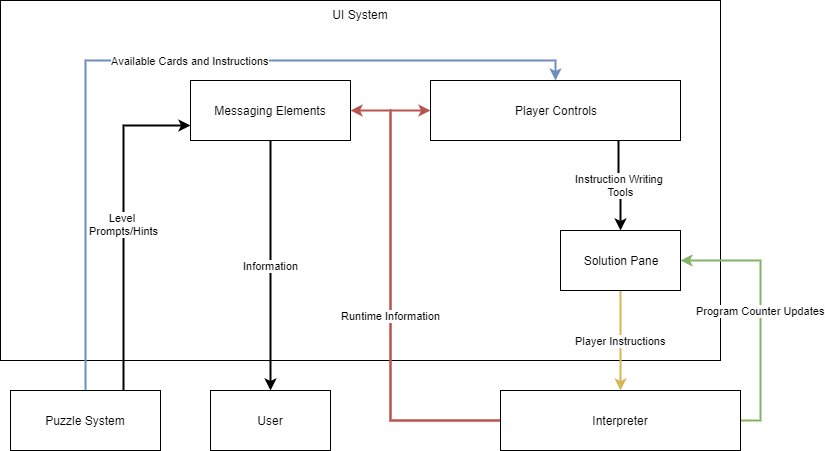
\includegraphics[width=\textwidth]{Diagrams/UI_Overview.png}
\end{figure}

\subsubsection{Player Controls}

As the player engages with the game, they will be able to control the simulation of their solution as it is executed in the puzzle game space. Once the player is ready to test out a solution, they will press a button to begin execution. At this point, the interpreter will get the instructions from the UI and determine the sequence of steps that will be simulate the solution. This gets communicated to the actor to determine the moves it will take across the game space. As the actor progresses through its actions, it communicates with the UI to grab data from UI elements and move data to other UI elements. These simulation steps cannot just be discarded once they are completed, since the player has controls to pause the simulation, proceed, or rewind to previous steps. These player controls will require the UI to communicate with the actor, so that the actor knows if it should continue with the next action, stop, or rewind the previous action.

\subsubsection{Solution Pane}

The solution pane is where the player must utilize available instructions to construct a solution to the current puzzle. The set of available instructions is received from the puzzle system to the UI. When the player is ready to execute their solution, the sequence of instruction commands is sent to the interpreter to analyze and decide what actions will be taken. The location of this element in the puzzle scene can be seen in our unified prototype (Figure \ref{fig:Unified_Prototype}).

\subsubsection{Player Messaging}

Controlling the flow of information to the player presents both technical and design issues to the team. Providing too many hints, prompts, and explanations can quickly turn the game into a glorified textbook; however, providing too few will make the game feel frustrating and inaccessible to our target audience. The User Interface will be tasked with handling this complex problem space.   

For the UI to be capable of delivering relevant information to the player, it must communicate with other major game systems. The Puzzle System's data-driven approach will allow it to provide the UI with puzzle specific data for each level of the game. Hints, prompts, and descriptions to be displayed to the player can all be retrieved from the Puzzle System on level start-up. Removing the responsibility of managing what information to display will allow the UI Designer to focus on player controls, and regulating the flow of information to the player.

In addition to its interactions with the Puzzle System, the User Interface will also communicate with the Interpreter to capture and display runtime information to the player. Common communications include runtime errors, program counter updates, or messages to reflect conditions that arise during execution executing.
